% Login

È possibile accedere alla propria area personale solo se si è registrati alla piattaforma (per registrarsi alla piattaforma, seguire i passaggi illustrati nel paragrafo \S{4}. La registrazione a Sweeat è gratuita e disponibile a chiunque).

È possibile accedere al modulo di accesso tramite il seguente link:

\begin{center}
\textsl{ \href{https://dev.d1ay0almkohcfw.amplifyapp.com/login}{\textbf{https://dev.d1ay0almkohcfw.amplifyapp.com/login} }}
\end{center}

Accedere alla propria Area Personale è molto semplice; dopo aver cliccato sul bottone “\textbf{Accedi}” nella barra di navigazione (in alto a destra nella versione Desktop e dal menù a tendina nella versione mobile), l’utente verrà reindirizzato in una nuova pagina.

\begin{figure}[H]
\centering

\includegraphics[scale=0.15]{./images/Login/LoginDesktop.png} 
\caption{Bottone di accesso versione desktop}
\end{figure}

\begin{figure}[H]
\centering
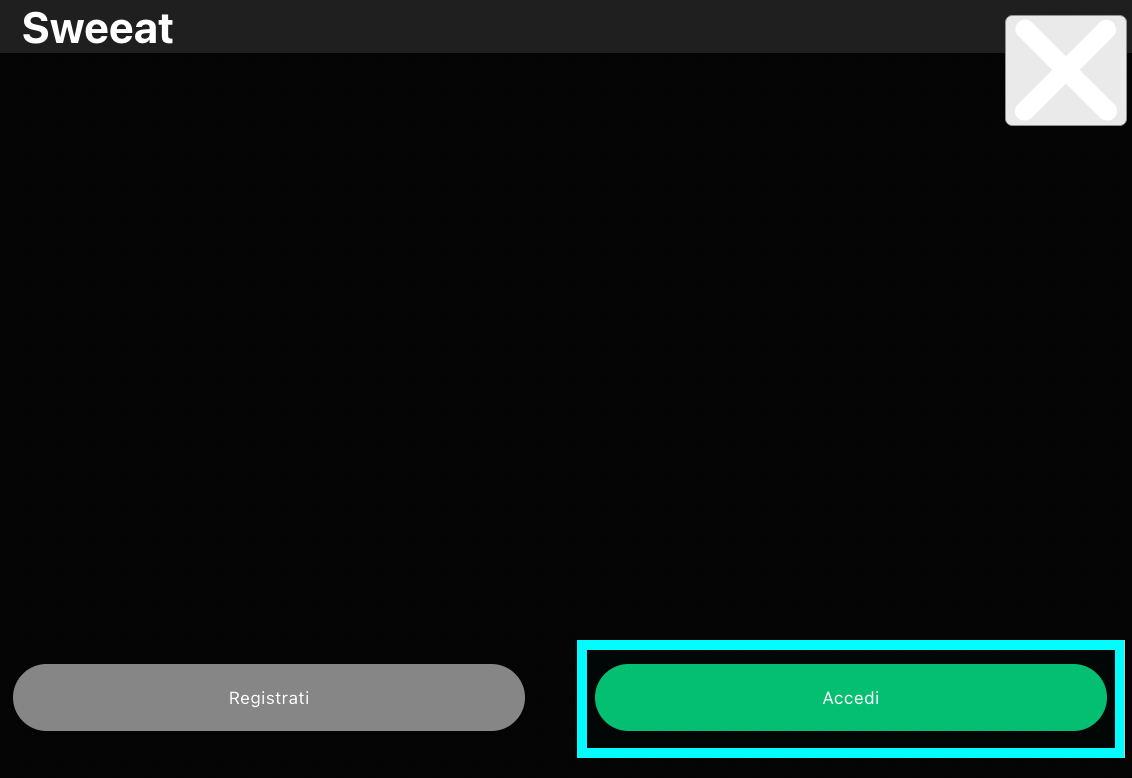
\includegraphics[scale=0.2]{./images/Login/LoginMobile.png} 
\caption{Bottone di accesso versione mobile}
\end{figure}

In questa nuova pagina comparirà un modello da compilare, nel quale l’utente dovrà inserire i seguenti dati personali:

\begin{enumerate}
\item \textbf{Indirizzo e-mail},
\item \textbf{Password}.
\end{enumerate}

\begin{figure}[H]
\centering
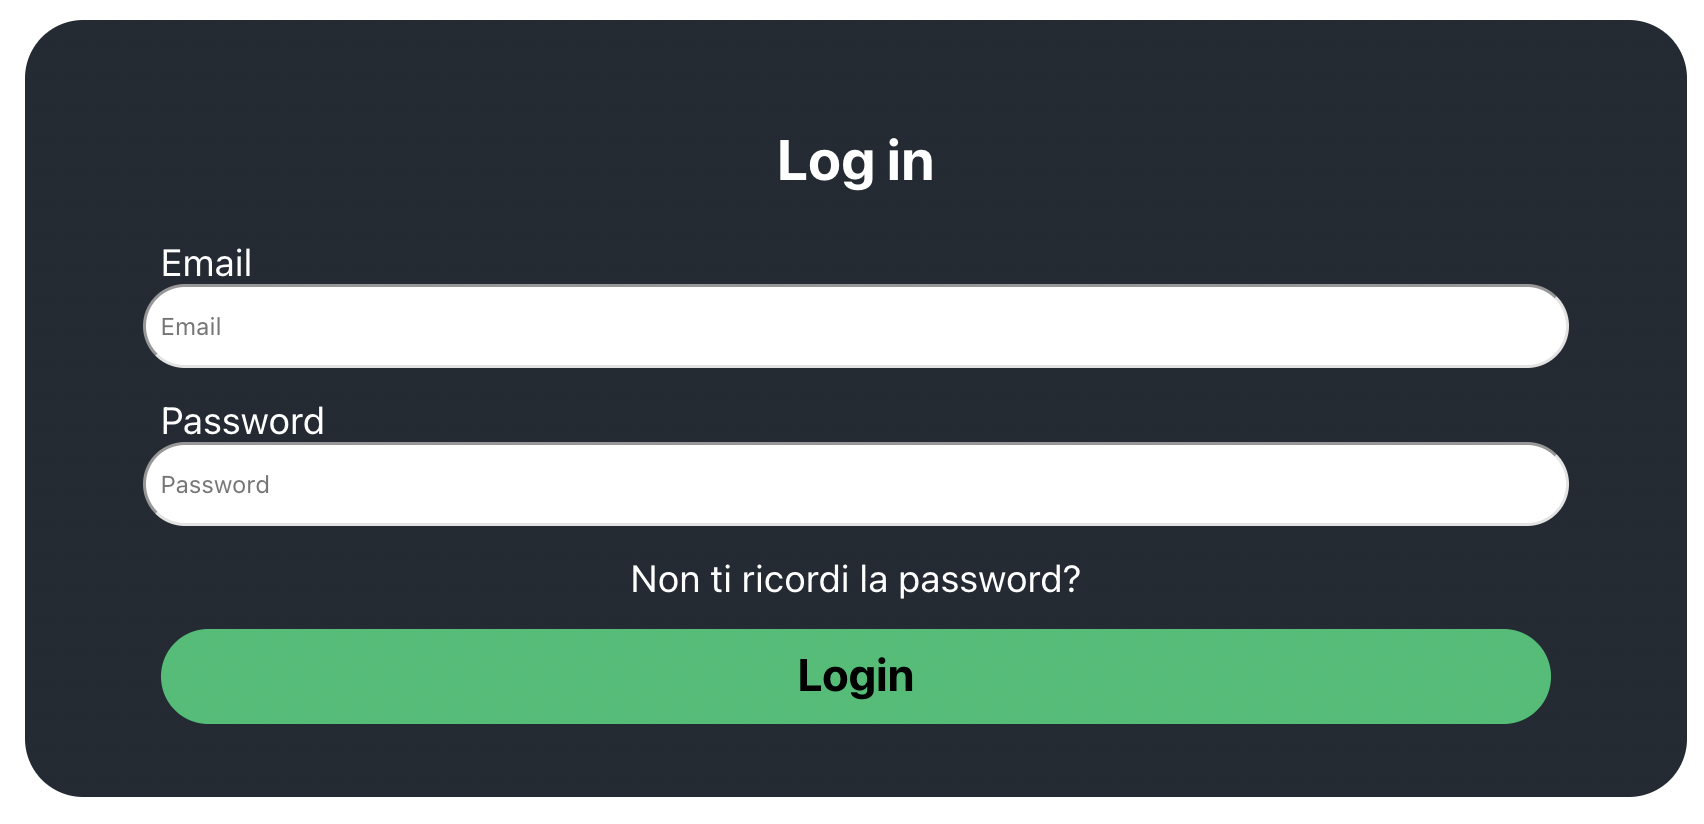
\includegraphics[scale=0.3]{./images/Login/FormLogin.png} 
\caption{Modulo di accesso da compilare per accedere a Sweeat}
\end{figure}

Entrambi i campi sono obbligatori ed i dati sono quelli inseriti in fase di registrazione (\S{4}). 

Una volta inseriti i dati, per accedere all’area personale sarà sufficiente cliccare sul bottone “\textbf{Login}”.

Dopo aver effettuato l’accesso, sarà possibile navigare nella propria \textbf{Area Personale}.

\subsection{Inserimento credenziali errate}

Nel caso in cui l'utente non inserisca le credenziali di accesso nel form di login, compariranno i seguenti errori: 

\begin{figure}[H]
\centering
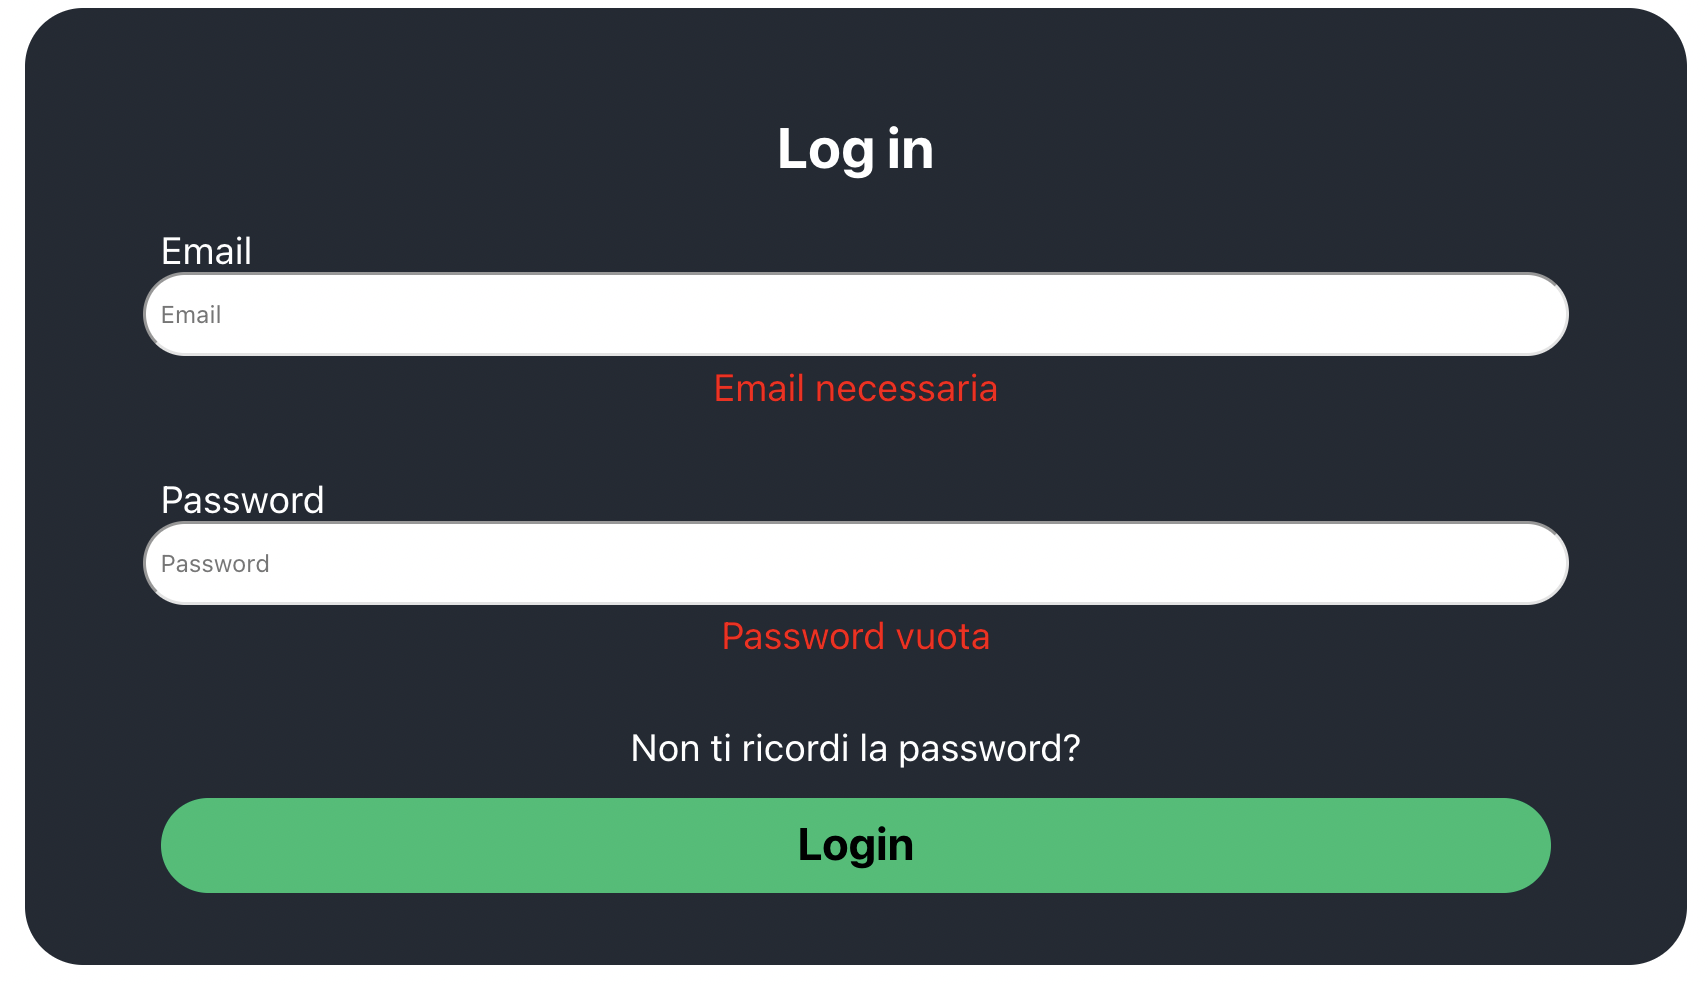
\includegraphics[scale=0.3]{./images/Login/ErroreCampi.png} 
\caption{Credenziali per il login non inserite}
\end{figure}

Per procedere, è necessario inserire le credenziali di accesso inserite in fase di registrazione (\S{4}), oppure procedere con il recupero password (\S{6}). 

Analogamente, nel caso in cui l'utente non inserisca delle credenziali corrette, all'utente verrà mostrato il seguente errore:

\begin{figure}[H]
\centering
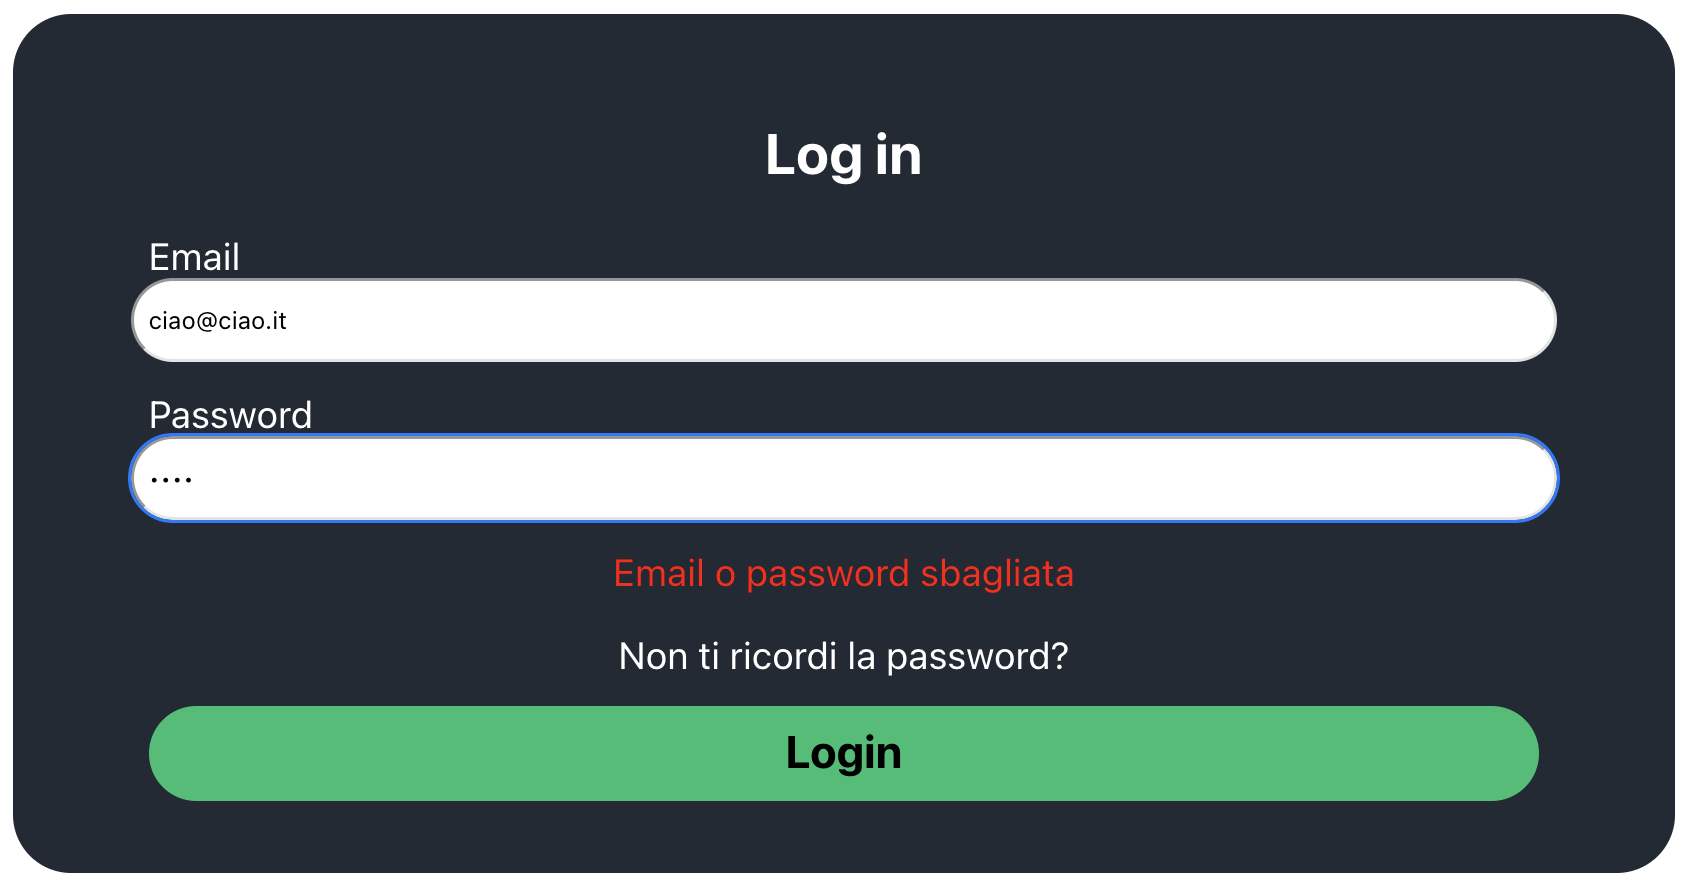
\includegraphics[scale=0.3]{./images/Login/AccessoNegato.png} 
\caption{Errore nell'inserimento delle credenziali per effettuare l'accesso}
\end{figure}

\subsection{Logout}

Un utente che ha effettuato l'accesso nella piattaforma, può “sloggarsi” cliccando sulla voce “\textbf{Log out}” presente nella barra di navigazione in ogni pagina del sito.

\begin{figure}[H]
\centering

\includegraphics[scale=0.15]{./images/Login/Logout.png} 
\caption{Logout da Sweeat}
\end{figure}

Se l'utente non ricorda più la password di accesso, potrà recuperarla tramite l'operazione di recupero password (\S{6}).